% Apresentações em widescreen. Outros valores possíveis: 1610, 149, 54, 43 e 32.
% Por padrão, as apresentações são no formato 4:3 (sem o aspectratio).
\documentclass[aspectratio=169]{beamer}	 	

\usetheme{Berkeley}
\usecolortheme{default}
\usefonttheme[onlymath]{serif}			% para fontes matemáticas

% ---
% PACOTES
% --
\usepackage[alf]{abntex2cite}		% Citações padrão ABNT
\usepackage[brazil]{babel}		    % Idioma do documento
\usepackage{color}			       % Controle das cores
\usepackage[T1]{fontenc}		  % Selecao de codigos de fonte.
\usepackage{graphicx}			    % Inclusão de gráficos
\usepackage[utf8]{inputenc}		   % Codificacao do documento (conversão automática dos acentos)
\usepackage{multirow}
\usepackage{threeparttable}
\usepackage[capposition=top]{floatrow}
\usepackage{txfonts}			 % Fontes virtuais
\usepackage{ragged2e}
\usepackage{etoolbox}
\usepackage{lipsum}
\usepackage{amssymb}
% ---

% ---
% Minhas Definições
% ---

%Deixando o Caption alinhado a esquerda mesmo com quebra de linha
\usepackage[labelfont=bf, justification=justified,singlelinecheck=true]{caption}

%Justificando o corpo do texto
\renewcommand{\raggedright}{\leftskip=0pt \rightskip=0pt plus 0cm} 

% Colocando numero de paginas no slide
\setbeamertemplate{footline}[frame number]{}
\setbeamertemplate{caption}[numbered]{}

% Tela cheia
%\hypersetup{pdfpagemode=FullScreen}
% ---


% --- Informações do documento ---
\logo{
\includegraphics[scale=0.15]{figuras/logo.png}}
\title{Ambiente Virtual de Aprendizagem para Auxiliar no Processo de Ensino e Aprendizagem de Matemática}
\author[]{Marciano Machado Saraiva}
\institute{
Orientador: Prof. Me. Samy Soares Passos de Sá\\[2 ex]
Universidade Federal do Ceará
	    \par
	    Bacharel em Sistemas de Informação}
\date{\today}
% ---

% ----------------- INÍCIO DO DOCUMENTO --------------------------------------
\begin{document}

% ----------------- NOVO SLIDE --------------------------------
\begin{frame}

    \titlepage

\end{frame}

% ----------------- NOVO SLIDE --------------------------------
% \begin{frame}{Roteiro}
%	\tableofcontents
%\end{frame}

%% ----------------- NOVO SLIDE --------------------------------
\section{Introdução}

\begin{frame}{Introdução}
\framesubtitle{Motivação}

\begin{itemize}
	\item Grande número de reprovações e desistências em turmas iniciais de Matemática de cursos na Universidade Federal do Ceará - Campus Quixadá.
	\item A Organização para Cooperação e Desenvolvimento Econômico(OECD) revelou que em 2015, 67.1\% do alunos brasileiros est\~ao abaixo do nível 2 (os níveis vão de 1 a 6) na escala do 
PISA \cite{pisainfocus2016}.

\end{itemize}

\end{frame}

% ----------------- NOVO SLIDE --------------------------------
\begin{frame}
\frametitle{Introdução}
\framesubtitle{Objetivos}

\begin{block}{Objetivo Geral}
	Desenvolver um Ambiente Virtual de Aprendizagem para auxiliar no processo de ensino e aprendizagem de matemática por alunos dentro e fora da sala de aula.
	\pause
\end{block}

\begin{block}{Objetivos Específicos}
  \begin{itemize}
  \item Levantar os requisitos do sistema.
  \pause
  \item Desenvolver os módulos com funções de administração do sistema.
  \pause
  \item Desenvolver os módulos com funções que serão utilizadas pelos estudantes aplicando técnicas de Gamificação.
  \pause
  \item Verificar a influência e impactos provocados pelo AVA no aprendizado de alunos em turmas de matem\'atica da Universidade Federal do Ceará.
\end{itemize}
\end{block}

\end{frame}

% ----------------- NOVO SLIDE --------------------------------
\section{Revisão Bibliográfica}

\begin{frame}{Revisão Bibliográfica}

\begin{itemize}
\item Metodologias no Ensino da Matemática
	\begin{itemize}
		\item Aula Expositiva
		\item Resolução de Problemas
		\item Modelagem Matemática
		\item O uso de computadores
	\end{itemize}
\item Ambiente Virtual de Aprendizagem
\item Gamifica\c{c}\~ao
	\begin{itemize}
	\item[$\longrightarrow$] Sistema de Pontua\c{c}\~ao
	\item[$\longrightarrow$] Rankings
	\item[$\longrightarrow$] N\'iveis
	\item[$\longrightarrow$] Personalização
	\end{itemize}

\end{itemize}


\end{frame}

% ----------------- NOVO SLIDE --------------------------------
\begin{frame}{Trabalhos Relacionados}
\frametitle{Revisão Bibliográfica}
\framesubtitle{Trabalhos Relacionados}

\begin{overprint}

\only<+>{

\begin{block}{The one world schoolhouse: Education reimagined}
	A Khan Academy tem como objetivo oferecer exercícios, vídeos de instrução e um painel de aprendizado personalizado que habilita os estudantes a aprender no seu próprio ritmo.
	\begin{itemize}
	\item[$\longrightarrow$] Aprendizagem auto-ritmada
	\item[$\longrightarrow$] O professor possui o papel de facilitador
	\end{itemize}
\end{block}
}
\only<+>{
\begin{block}{ActiveMath: A generic and adaptive web-based learning environment}
O projeto ActiveMath visa apoiar a aprendizagem verdadeiramente interativa e exploratória.
	\begin{itemize}
	\item[$\longrightarrow$] Cursos gerados dinamicamente a partir de regras pedagógicas
	\item[$\longrightarrow$] Diagnósticos de erros e equívocos dos estudantes, que gera estratégias tutoriais configuráveis para o \textit{feedback}
	\end{itemize}
\end{block}

}
\only<+>{

\begin{block}{Duolingo: Learn a Language for Free while Helping to Translate the Web}
O Duolingo \'e uma plataforma de ensino de idiomas e tradução automática de documentos.
	\begin{itemize}
	\item[$\longrightarrow$] Utiliza lições fragmentadas, pelas quais os alunos, através do método de repetição, fixam o conteúdo estudado
	\end{itemize}
\end{block}
}

\only<+>{
\begin{block}{Resolução de problemas em ambientes virtuais de aprendizagem num curso de licenciatura em matemática na modalidade a distância}
	\begin{itemize}
	\item[$\longrightarrow$] A atividade é postada na Plataforma Moodle no início da semana
	\item[$\longrightarrow$] Os alunos passam a semana postando suas resoluções dos problemas num fórum de discussão
	\end{itemize}

\end{block}

}
\end{overprint}


\end{frame}

% ----------------- NOVO SLIDE --------------------------------
\section{Descrição da Proposta}

\setcounter{figure}{0}

\begin{frame}{Descrição da Proposta}

\begin{overprint}
\only<+>{
	\begin{figure}[H]
	\centering
	\caption{Representa\c{c}\~ao do nosso Modelo de Aprendizagem}
	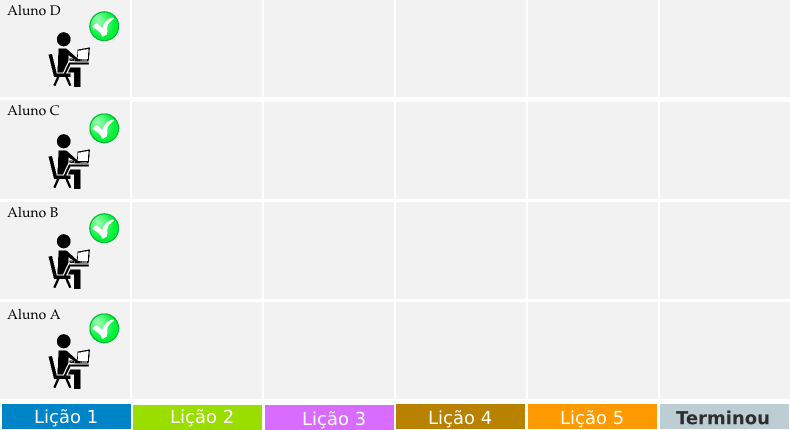
\includegraphics[width=8cm]{figuras/proposta/imagem1.png}
	\floatfoot{Fonte: Elaborada pelo autor}
	\end{figure}
}
\only<+>{
	\begin{figure}[H]
	\centering
	\caption{Representa\c{c}\~ao do nosso Modelo de Aprendizagem}
	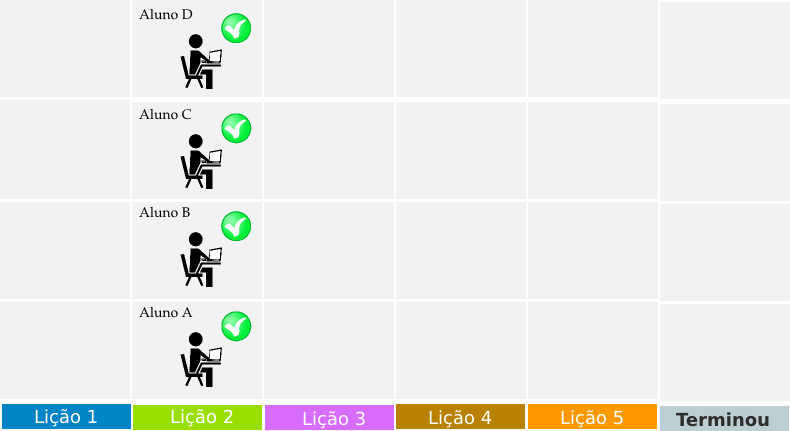
\includegraphics[width=8cm]{figuras/proposta/imagem2.png}
	\floatfoot{Fonte: Elaborada pelo autor}
	\end{figure}
}
\only<+>{
	\begin{figure}[H]
	\centering
	\caption{Representa\c{c}\~ao do nosso Modelo de Aprendizagem}
	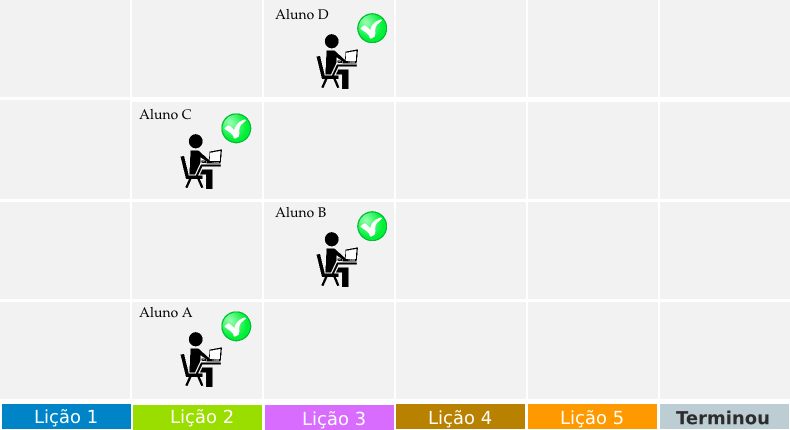
\includegraphics[width=8cm]{figuras/proposta/imagem3.png}
	\floatfoot{Fonte: Elaborada pelo autor}
	\end{figure}
}
\only<+>{
	\begin{figure}[H]
	\centering
	\caption{Representa\c{c}\~ao do nosso Modelo de Aprendizagem}
	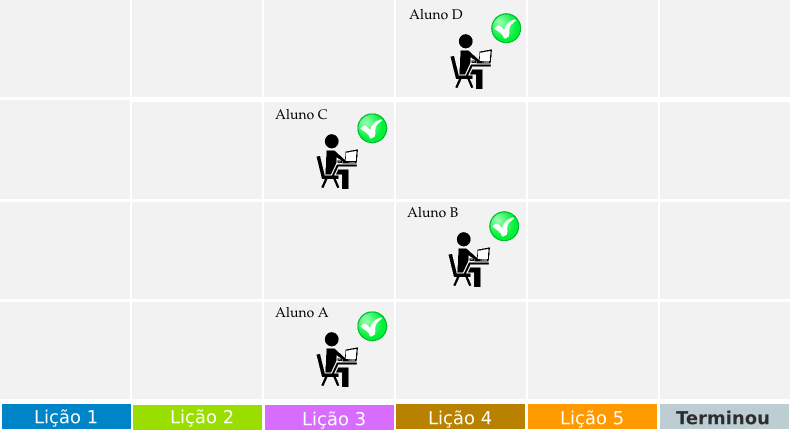
\includegraphics[width=8cm]{figuras/proposta/imagem4.png}
	\floatfoot{Fonte: Elaborada pelo autor}
	\end{figure}
}
\only<+>{
	\begin{figure}[H]
	\centering
	\caption{Representa\c{c}\~ao do nosso Modelo de Aprendizagem}
	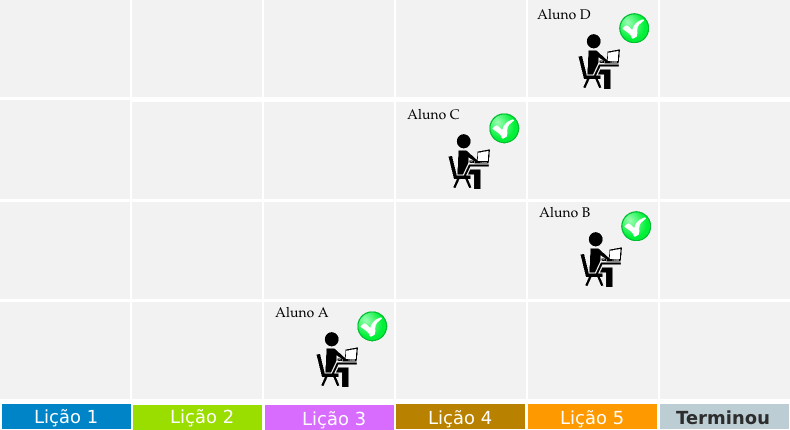
\includegraphics[width=8cm]{figuras/proposta/imagem5.png}
	\floatfoot{Fonte: Elaborada pelo autor}
	\end{figure}
}
\only<+>{
	\begin{figure}[H]
	\centering
	\caption{Representa\c{c}\~ao do nosso Modelo de Aprendizagem}
	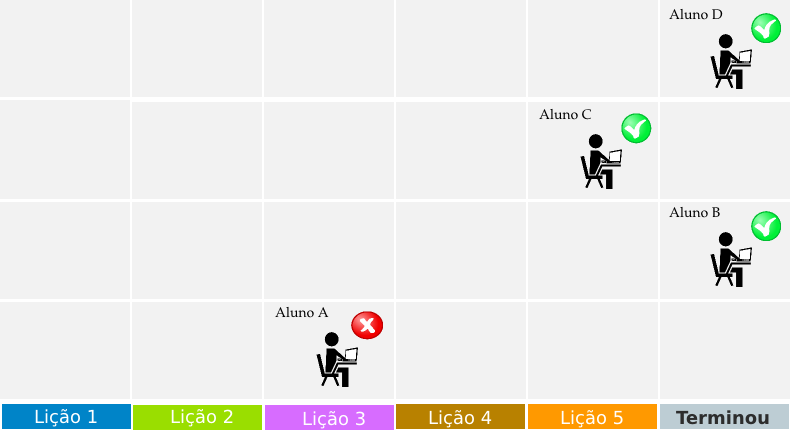
\includegraphics[width=8cm]{figuras/proposta/imagem6.png}
	\floatfoot{Fonte: Elaborada pelo autor}
	\end{figure}
}
\only<+>{
	\begin{figure}[H]
	\centering
	\caption{Representa\c{c}\~ao do nosso Modelo de Aprendizagem}
	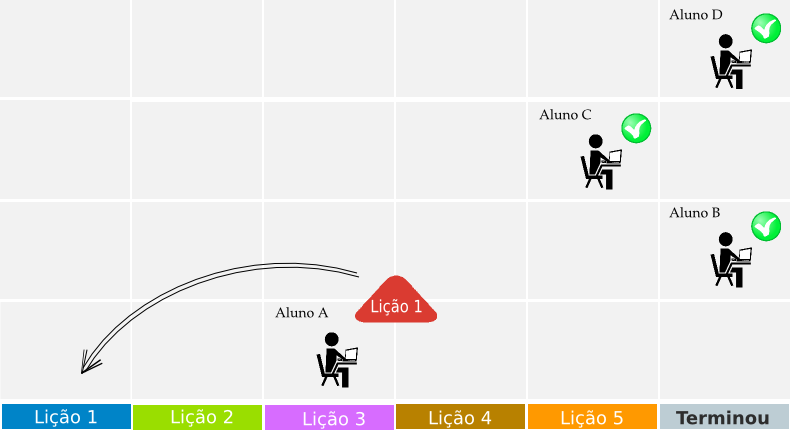
\includegraphics[width=8cm]{figuras/proposta/imagem7.png}
	\floatfoot{Fonte: Elaborada pelo autor}
	\end{figure}
}
\only<+>{
	\begin{figure}[H]
	\centering
	\caption{Representa\c{c}\~ao do nosso Modelo de Aprendizagem}
	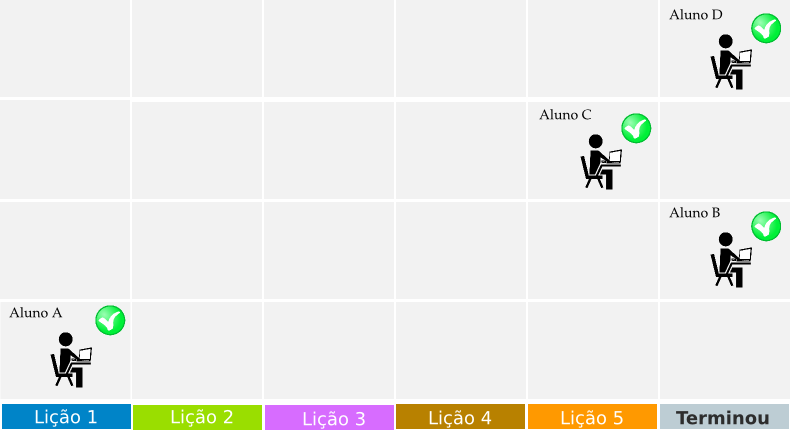
\includegraphics[width=8cm]{figuras/proposta/imagem8.png}
	\floatfoot{Fonte: Elaborada pelo autor}
	\end{figure}
}
\only<+>{
	\begin{figure}[H]
	\centering
	\caption{Representa\c{c}\~ao do nosso Modelo de Aprendizagem}
	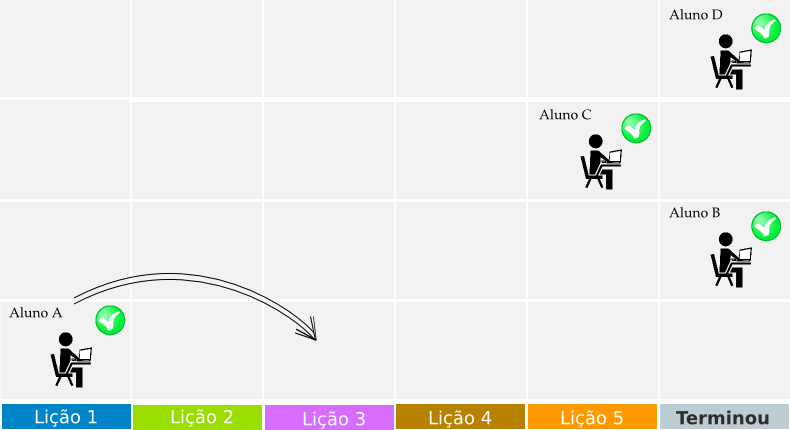
\includegraphics[width=8cm]{figuras/proposta/imagem9.png}
	\floatfoot{Fonte: Elaborada pelo autor}
	\end{figure}
}
\only<+>{
	\begin{figure}[H]
	\centering
	\caption{Representa\c{c}\~ao do nosso Modelo de Aprendizagem}
	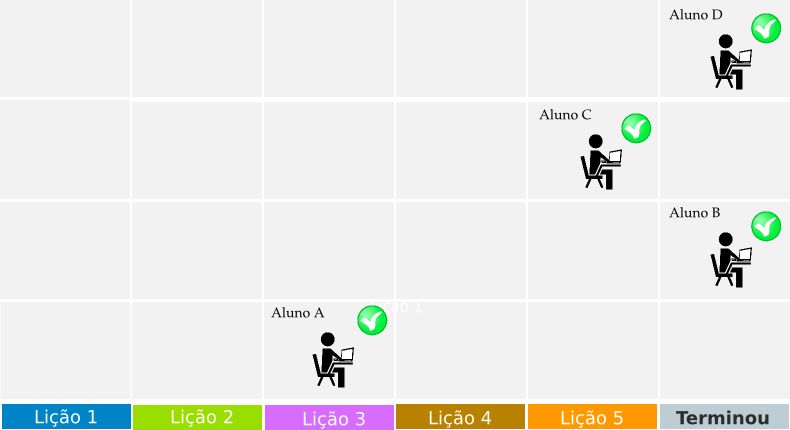
\includegraphics[width=8cm]{figuras/proposta/imagem10.png}
	\floatfoot{Fonte: Elaborada pelo autor}
	\end{figure}
}

\only<+>{
	\begin{figure}[H]
	\centering
	\caption{Representa\c{c}\~ao do nosso Modelo de Aprendizagem}
	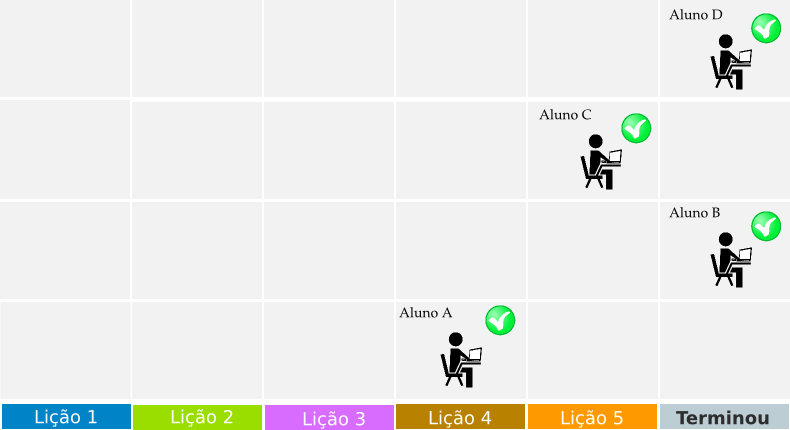
\includegraphics[width=8cm]{figuras/proposta/imagem11.png}
	\floatfoot{Fonte: Elaborada pelo autor}
	\end{figure}
}

\only<+>{
	\setcounter{figure}{1}
	\begin{figure}[H]
	\centering
	\caption{Estrutura do Problema}
	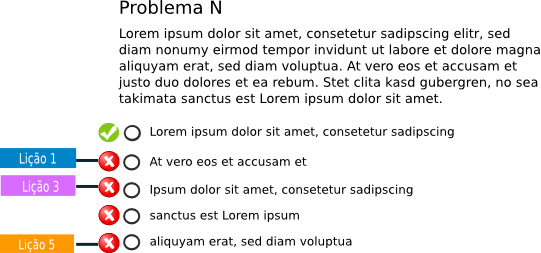
\includegraphics[width=8cm]{figuras/estrutura_problema.png}
	\floatfoot{Fonte: Elaborada pelo autor}
	\end{figure}
}

\only<+>{
	\begin{table}[H]
		\caption{Compara\c{c}\~ao entre os tradicionais modelos de aprendizagem e o nosso.}
		\resizebox{8cm}{!}{
			
			\begin{tabular}{|l|l|}
			\hline
			\textbf{Modelos Tradicionais}                                        & \textbf{Nosso Modelo}                                                 \\ \hline
			\begin{tabular}[c]{@{}l@{}}Centrado no professor\end{tabular}      & Centrado no aluno                                                     \\ \hline
			\begin{tabular}[c]{@{}l@{}}Absorção passiva\end{tabular}           & \begin{tabular}[c]{@{}l@{}}Participação ativa do aluno\end{tabular} \\ \hline
			O professor como especialista                                        & O professor como guia                                                 \\ \hline
			Estático                                                             & Dinâmico                                                              \\ \hline
			\begin{tabular}[c]{@{}l@{}}Aprendizado predeterminado\end{tabular} & \begin{tabular}[c]{@{}l@{}}Aprender a aprender\end{tabular}         \\ \hline
			\end{tabular}
		
		}
		\floatfoot{Fonte: Elaborada pelo autor}
	\end{table}
}


\end{overprint}

\end{frame}

% ----------------- NOVO SLIDE --------------------------------
\section{Procedimentos Metodológicos}

\begin{frame}{Procedimentos Metodológicos}
	\begin{enumerate}
    	\item Definição do Processo
        \item Levantamento e Análise de Requisitos
        \item Projeto do Sistema
        \item Implementação do Sistema
        \item Verificação e Validação
        \item Definição do Conteúdo para o Sistema
        \item Aplicação da Solução na Universidade Federal do Ceará - Campus Quixadá
    \end{enumerate}
\end{frame}

% ----------------- NOVO SLIDE --------------------------------

\begin{frame}{Procedimentos Metodológicos}
\frametitle{Procedimentos Metodológicos}
\framesubtitle{Definição do Processo}


\end{frame}

% ----------------- NOVO SLIDE --------------------------------

\begin{frame}{Procedimentos Metodológicos}
\frametitle{Procedimentos Metodológicos}
\framesubtitle{Levantamento e Análise de Requisitos}

\begin{overprint}

\only<+>{
	\begin{block}{P\'ublico-Alvo}
		\begin{itemize}
			\item Professores e Estudantes do Ensino M\'edio e Superior
		\end{itemize}
	\end{block}

}
\only<+>{
	\begin{block}{Principais Requisitos do Sistema}
		\begin{enumerate}
		\item Hierarquia dos Conteúdos
		\item Estrutura do Problema
		\item Saltar Problemas
		\item Pedir Ajuda
		\item Deficiências
		\item Fórum
		\end{enumerate}
	\end{block}

}

\end{overprint}

\end{frame}

% ----------------- NOVO SLIDE --------------------------------

\begin{frame}{Procedimentos Metodológicos}
\frametitle{Procedimentos Metodológicos}
\framesubtitle{Projeto do Sistema}

\begin{overprint}
\setcounter{figure}{2}
\only<+>{

\begin{block}{Arquitetura do Sistema}
	\begin{figure}[H]
	\centering
	\caption{Arquitetura do Sistema}
	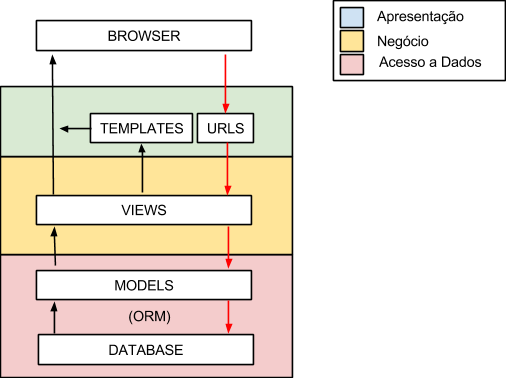
\includegraphics[width=5cm]{figuras/arquitetura.png}
	\floatfoot{Fonte: Elaborada pelo autor}
	\end{figure}
\end{block}

}
\only<+>{

\begin{block}{Ferramentas Utilizadas}
	\begin{itemize}
	  \item \textbf{Linguagem de Programa\c{c}\~ao}: Python
	  \item \textbf{Framework Back-end}: Django
	  \item \textbf{Framework Front-end}: Metro UI CSS
	  \item \textbf{Plugin de Internacionaliza\c{c}\~ao}: Rosetta
	  \item \textbf{Banco de Dados}: PostgreSQL
	  \item \textbf{Engine para Latex}: MathJax
	\end{itemize}
\end{block}

}

\end{overprint}


\end{frame}

% ----------------- NOVO SLIDE --------------------------------

\begin{frame}{Procedimentos Metodológicos}
\frametitle{Procedimentos Metodológicos}
\framesubtitle{Implementação do Sistema}

\begin{block}{Ambiente de Desenvolvimento}
	 \begin{itemize}
	  \item \textbf{Sistema Operacional}: Ubuntu 14.04 LTS
	  \item \textbf{Interpretador}: Python 2.7.6
	  \item \textbf{Banco de Dados}: PostgreSQL 9.3.13
	  \item \textbf{Framework de back-end}: DJango 1.7.11
	  \item \textbf{Framework de front-end}: Metro UI CSS 3.0.15
	  \item \textbf{Virtualiza\c{c}\~ao}: Virtualenv 15.0.2
	  \item \textbf{Controle de Vers\~ao}: Git 1.9.1
	 \end{itemize}

\end{block}


\end{frame}

% ----------------- NOVO SLIDE --------------------------------

\begin{frame}{Procedimentos Metodológicos}
\frametitle{Procedimentos Metodológicos}
\framesubtitle{Verificação e Validação}

\begin{block}{Testes que ser\~ao realizados}
	\begin{itemize}
	 \item \textbf{Teste de Unidade} – é aquele que testa uma única unidade do sistema.
	 \item \textbf{Teste de Integração} – é aquele que testa a integração entre duas ou mais partes de um sistema.
	 \item \textbf{Teste de Sistema} – é aquele que garante que o sistema funciona como um todo.
	\end{itemize}

\end{block}


\end{frame}

% ----------------- NOVO SLIDE --------------------------------

\begin{frame}{Procedimentos Metodológicos}
\frametitle{Procedimentos Metodológicos}
\framesubtitle{Definição do Conteúdo para o Sistema}
	\begin{itemize}
	 \item A aplicação da primeira versão do sistema ocorrer\'a em duas turmas de Matemática na Universidade
Federal do Ceará - Campus Quixadá.
	\item Os monitores dessas turmas passar\~ao por um treinamento, em que aprender\~ao a utilizar o sistema para assim, adicionarem os conte\'udos.
	\end{itemize}

\end{frame}

% ----------------- NOVO SLIDE --------------------------------

\setcounter{figure}{3}

\begin{frame}{Procedimentos Metodológicos}
\frametitle{Procedimentos Metodológicos}
\framesubtitle{Aplicação da Solução na Universidade Federal do Ceará - Campus Quixadá}

\begin{figure}[H]
\centering
\caption{Turmas em que o sistema ser\'a aplicado}
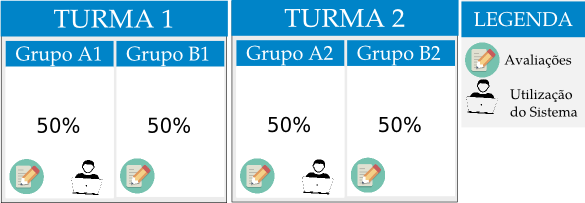
\includegraphics[width=10cm]{figuras/aplicacao.png}
\floatfoot{Fonte: Elaborada pelo autor}
\end{figure}

\end{frame}

% ----------------- NOVO SLIDE --------------------------------

\begin{frame}{Procedimentos Metodológicos}
\frametitle{Procedimentos Metodológicos}
\framesubtitle{Cronograma}
	\begin{table}[H]
\centering
\caption{Cronograma de Execução}
\label{cronograma}

\resizebox{\textwidth}{!}{
\begin{tabular}{|l|c|c|c|c|c|c|c|c|c|c|c|c|c|c|c|}
\hline
\multicolumn{1}{|c|}{\multirow{2}{*}{ATIVIDADES}} & \multicolumn{6}{c|}{2015} & \multicolumn{9}{c|}{2016} \\ \cline{2-16} 
\multicolumn{1}{|c|}{} & Jan & Fev & Mar & Abr & Mai & Jun - Dez & \multicolumn{1}{l|}{Jan - Mar} & \multicolumn{1}{l|}{Abr} & \multicolumn{1}{l|}{Mai} & \multicolumn{1}{l|}{Jun} & \multicolumn{1}{l|}{Jul} & \multicolumn{1}{l|}{Ago} & \multicolumn{1}{l|}{Set} & \multicolumn{1}{l|}{Out} & \multicolumn{1}{l|}{Nov} \\ \hline
Definição do Processo & x &  &  &  &  &  &  &  &  &  &  &  &  &  &  \\ \hline
Levantamento e Análise dos Requisitos & x & x & x &  &  &  &  &  &  &  &  &  &  &  &  \\ \hline
Projeto do Sistema &  &  &  & x & x &  &  &  &  &  &  &  &  &  &  \\ \hline
Implementação do Sistema &  &  &  &  &  & x & x & x & x & x &  &  &  &  &  \\ \hline
Verificação e Validação &  &  &  &  &  &  &  &  &  &  & x &  &  &  &  \\ \hline
Desenvolver o conteúdo para o sistema &  &  &  &  &  &  &  & x & x & x & x & x &  &  &  \\ \hline
Aplicação na UFC - Campus Quixadá &  &  &  &  &  &  &  &  &  &  &  & x & x & x &  \\ \hline
Definição do Projeto de Pesquisa &  &  &  &  &  &  &  & x &  &  &  &  &  &  &  \\ \hline
Defesa do Projeto de Pesquisa &  &  &  &  &  &  &  &  &  & x &  &  &  &  &  \\ \hline
Ajustes Solicitados &  &  &  &  &  &  &  &  &  &  & x &  &  &  &  \\ \hline
Análise dos Resultados Obtidos na Aplicação. &  &  &  &  &  &  &  &  &  &  &  &  &  &  & x \\ \hline
Defesa do Trabalho Final &  &  &  &  &  &  &  &  &  &  &  &  &  &  & x \\ \hline
\end{tabular}}
\fnote{Fonte: Elaborado pelo autor}
\end{table}
\end{frame}


% ----------------- NOVO SLIDE --------------------------------
\section{Resultados Preliminares}
\begin{frame}{Resultados Preliminares}

\begin{overprint}

\only<1>{
	\begin{enumerate}
    	\item Definição do Processo 
\includegraphics[width=0.03\textwidth]{figuras/ok}
        \item Levantamento e Análise de Requisitos 
\includegraphics[width=0.03\textwidth]{figuras/ok}
        \item Projeto do Sistema 
\includegraphics[width=0.03\textwidth]{figuras/ok}
        \item Implementação do Sistema 
\includegraphics[width=0.03\textwidth]{figuras/deploy}
        \item Verificação e Validação
        \item Definição do Conteúdo para o Sistema 
\includegraphics[width=0.03\textwidth]{figuras/deploy}
        \item Aplicação da Solução na Universidade Federal do Ceará - Campus Quixadá
    \end{enumerate}
}

\only<2>{
Etapa de Implementação:
	\begin{columns}[t]
		\begin{column}{.425\textwidth}
			\begin{block}{Módulos Conclu\'idos}
				\begin{itemize}
					\item Gerenciador de Usuários
					\item Gerenciador de Turmas
					\item Gerenciador de Disciplinas
					\item Gerenciador de Lições
					\item Gerenciador de Problemas
					\item Gerenciador de Pontuação
					\item F\'orum
				\end{itemize}
			\end{block}
		\end{column}
		\begin{column}{.425\textwidth}  %%<--- here
			\begin{block}{Módulos em Desenvolvimento}
				\begin{itemize}
					\item Gerenciador de Progresso
					\item Gerador de Estatísticas
					\item Ranking
				\end{itemize}
			\end{block}
		\end{column}
	\end{columns}
}

\end{overprint}

\end{frame}

\begin{frame}{Resultados Preliminares}
	\begin{figure}[H]
	\centering
	\caption{Tela Inicial do Sistema}
	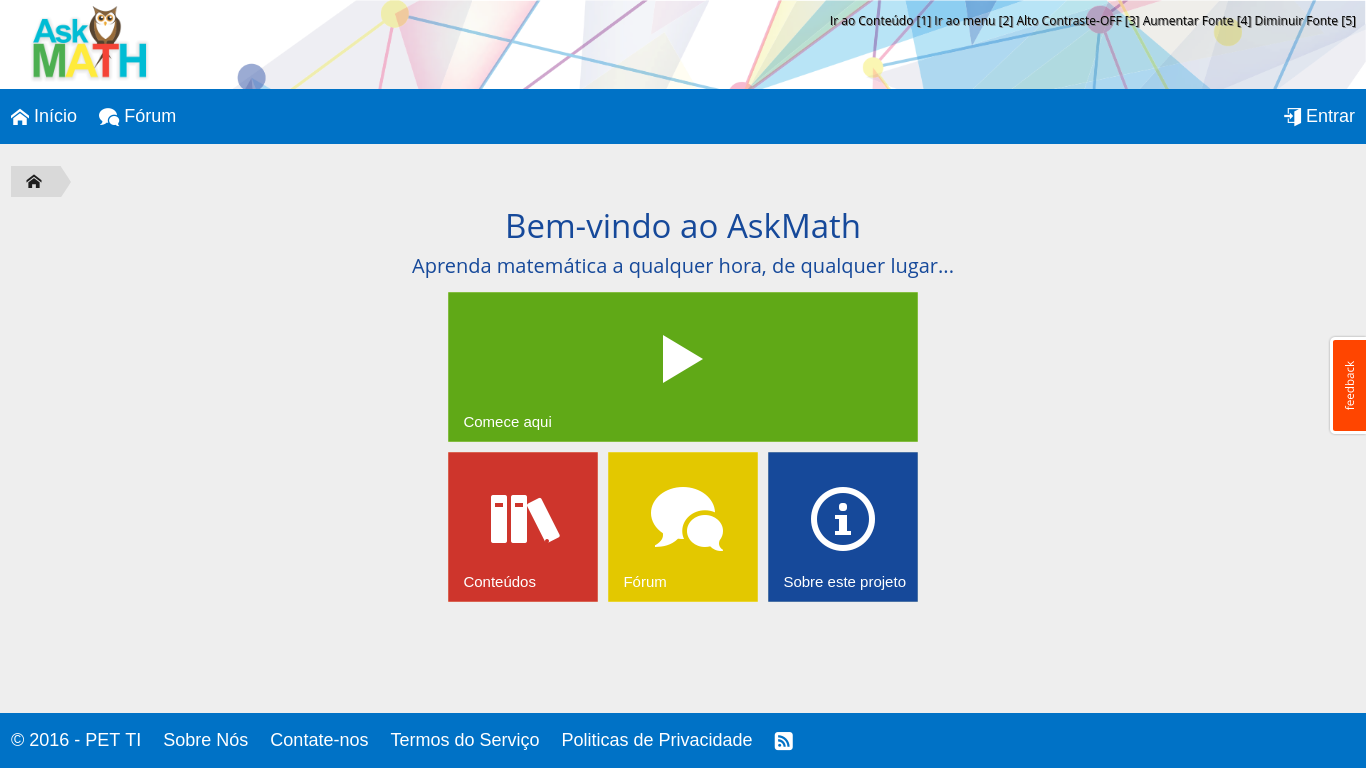
\includegraphics[width=8cm]{figuras/askmath/1.png}
	\floatfoot{Fonte: \url{www.askmath.quixada.ufc.br} }
	\end{figure}
\end{frame}

\begin{frame}{Resultados Preliminares}
	\begin{figure}[H]
	\centering
	\caption{Tela de Administra\c{c}\~ao do Sistema}
	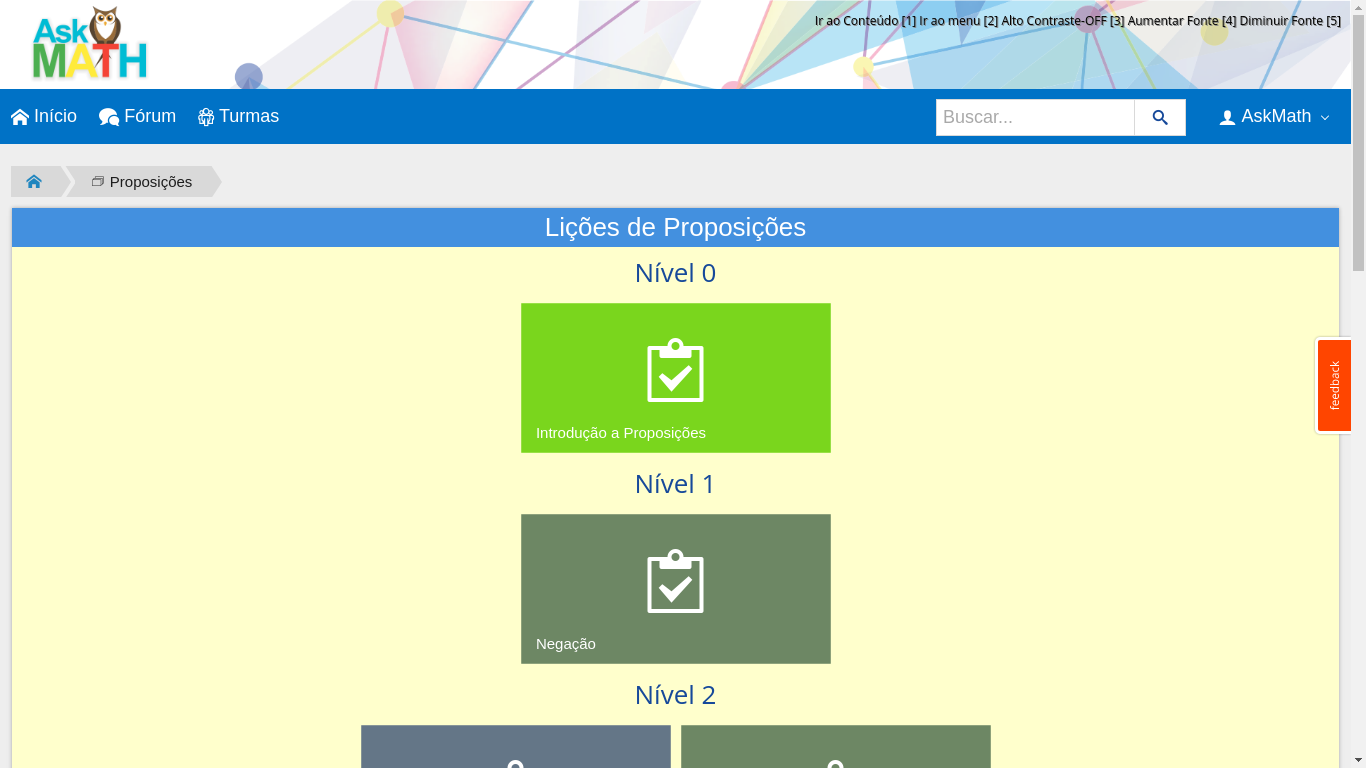
\includegraphics[width=8cm]{figuras/askmath/2.png}
	\floatfoot{Fonte: \url{www.askmath.quixada.ufc.br} }
	\end{figure}
\end{frame}

\begin{frame}{Resultados Preliminares}
	\begin{figure}[H]
	\centering
	\caption{Tela de Problemas do Aluno}
	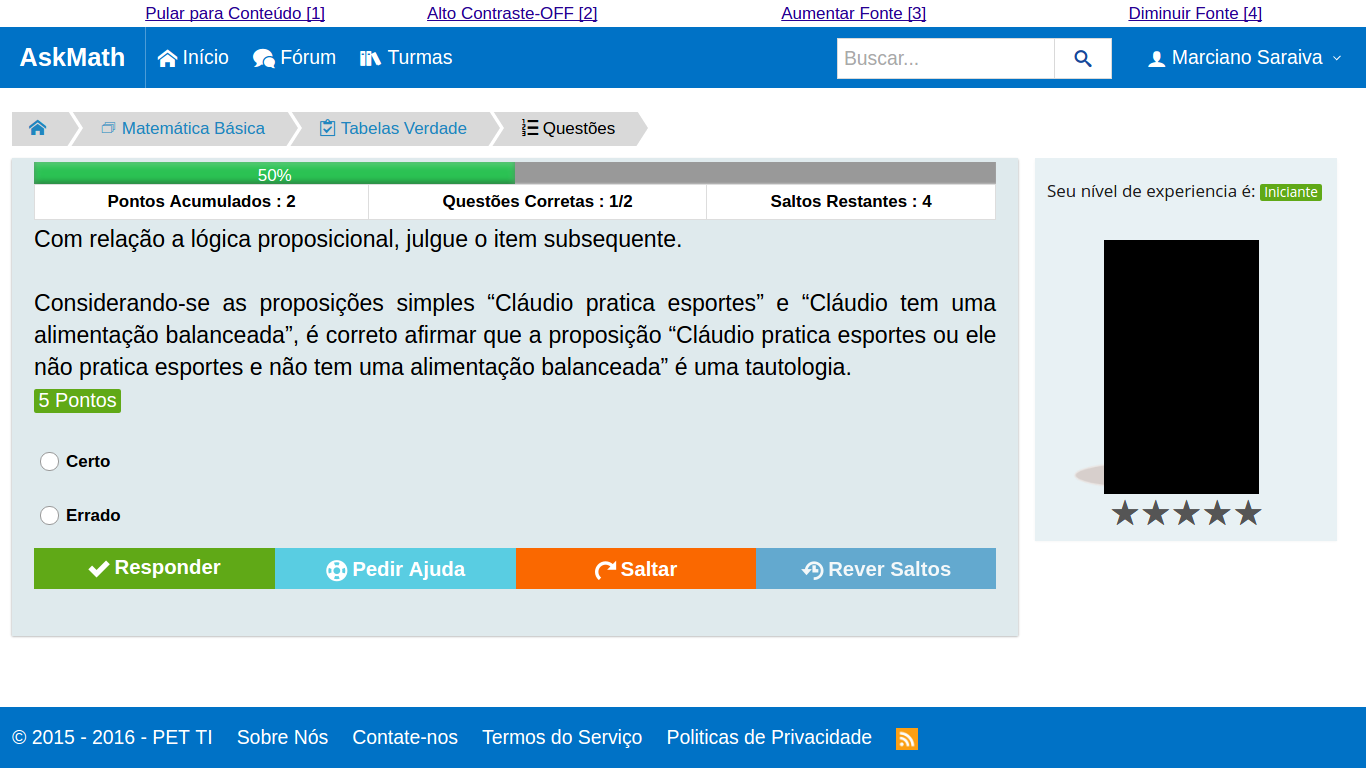
\includegraphics[width=8cm]{figuras/askmath/3.png}
	\floatfoot{Fonte: \url{www.askmath.quixada.ufc.br} }
	\end{figure}
\end{frame}

\begin{frame}{Resultados Preliminares}
	\begin{figure}[H]
	\centering
	\caption{Tela do F\'orum de Discuss\~oes}
	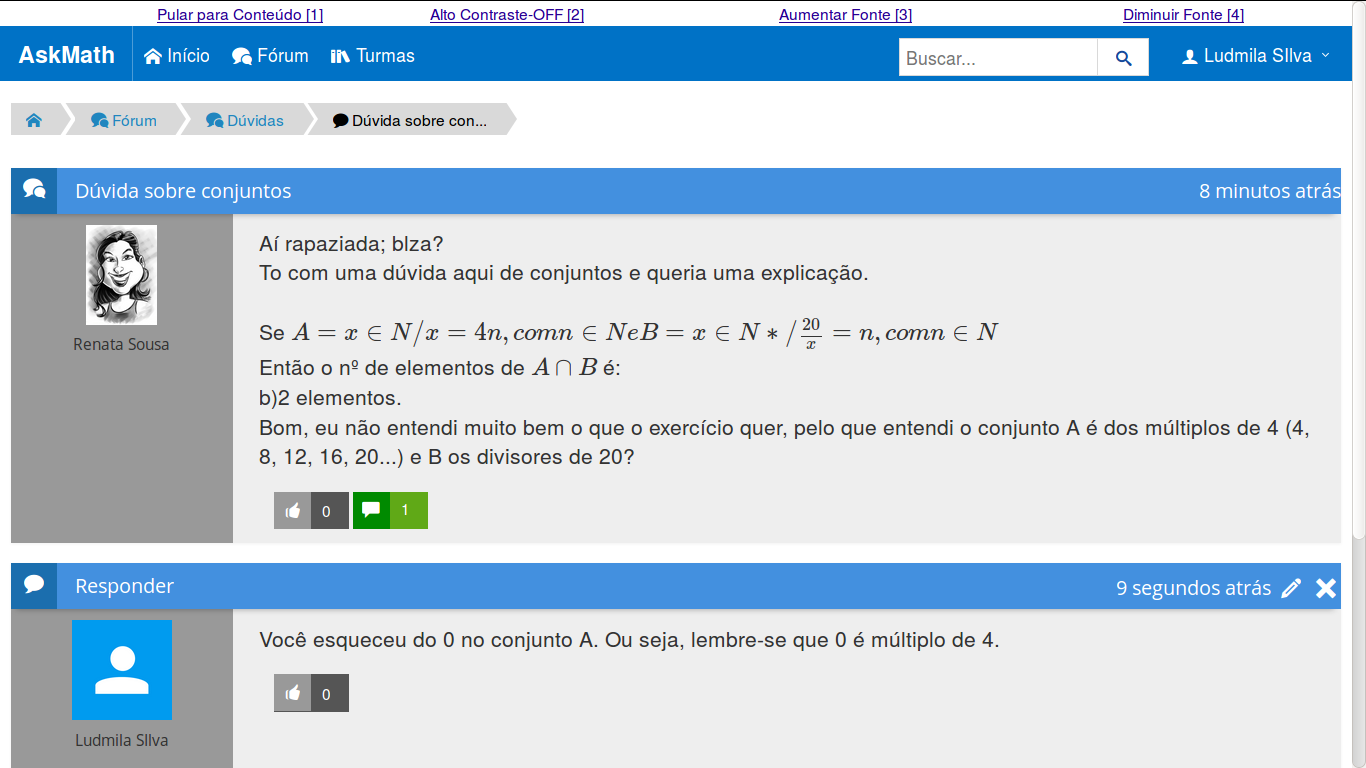
\includegraphics[width=8cm]{figuras/askmath/4.png}
	\floatfoot{Fonte: \url{www.askmath.quixada.ufc.br} }
	\end{figure}
\end{frame}

% ----------------- NOVO SLIDE --------------------------------
\section{Referências}

\begin{frame}[allowframebreaks]{Referências}
	\bibliography{referencias}
\end{frame}

% ----------------- NOVO SLIDE --------------------------------

\section{Coment\'arios}

\begin{frame}
	\begin{columns}
		\begin{column}{3cm}
			
\includegraphics[height=3cm]{figuras/logo.png}
		\end{column}
		\begin{column}{7cm}
			\begin{flushright}
				\centering
				\vskip 0.5cm
				\Huge Obrigado!
			\end{flushright}
		\end{column}
	\end{columns}
\end{frame}


% ----------------- FIM DO DOCUMENTO -----------------------------------------
\end{document}